\documentclass[9pt,t]{beamer}
\usetheme{Madrid}
\usepackage{amsthm, hhline}
\usepackage{stmaryrd, mathtools, stmaryrd}
\usepackage{amsmath, amssymb, graphicx,array}
\usepackage{mathtools}
\DeclareMathOperator{\lcm}{lcm}
\usepackage{booktabs,comment,bbm}
\newcommand{\Z}{\mathbb{Z}}
\newcommand{\N}{\mathbb{N}}
\usepackage[english]{babel}
\usepackage[utf8x]{inputenc}
\usepackage{color}
\usepackage[export]{adjustbox}
\setbeamerfont{title in sidebar}{size=\fontsize{2}{4}\selectfont}
\setbeamerfont{author in sidebar}{size=\fontsize{2}{4}\selectfont}
\setbeamerfont{section in sidebar}{size=\fontsize{2}{4}\selectfont}
\setbeamerfont{subsection in sidebar}{size=\fontsize{2}{4}\selectfont}
\newtheorem{proposition}[theorem]{Proposition}
\fontsize{6pt}{7.2}
\DeclareMathOperator{\ex}{\mathbb{E}}
\DeclareMathOperator{\pr}{\mathbb{P}}
\DeclareMathOperator{\indic}{\mathbbm{1}}
\DeclareMathOperator{\cov}{cov}
\DeclareMathOperator{\var}{var}
\DeclareMathOperator{\sgn}{sgn}
\DeclarePairedDelimiter\ceil{\lceil}{\rceil}
\DeclarePairedDelimiter\floor{\lfloor}{\rfloor}
\DeclarePairedDelimiter\abs{\lvert}{\rvert}


\title{Asymptotics of Bernoulli Line Ensembles}

\author[Fang, Fesser, Serio, Teitler, and Wang]{Xiang Fang, Lukas Fesser, Christian Serio, Carson Teitler, and Angela Wang \\
Advisor: Evgeni Dimitrov\\
Graduate Student Assistant: Weitao Zhu}

\institute[Columbia]{Columbia University REU}

\begin{document}
	
	\begin{frame}
		\maketitle
	\end{frame}


\section{Introduction (5-6 min)}

\begin{frame}{The Gaussian universality class}
Gaussian universality (CLT, Donsker Theorem)
\begin{figure}
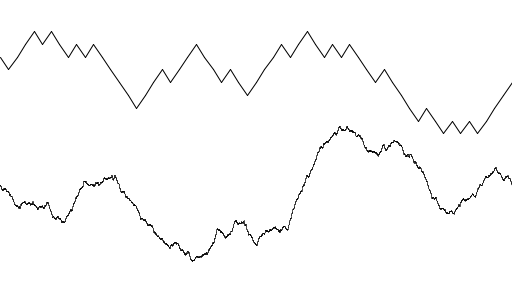
\includegraphics[height=0.5\textheight]{graphics/Gaussian.png}
\caption{An example of a Bernoulli random walk and a Brownian Motion}
\end{figure}

\end{frame}

\begin{frame}{Multiple Random Walks}
Increase the number of walkers (avoiding Bernoulli random walks and Dyson BM)
\begin{figure}
	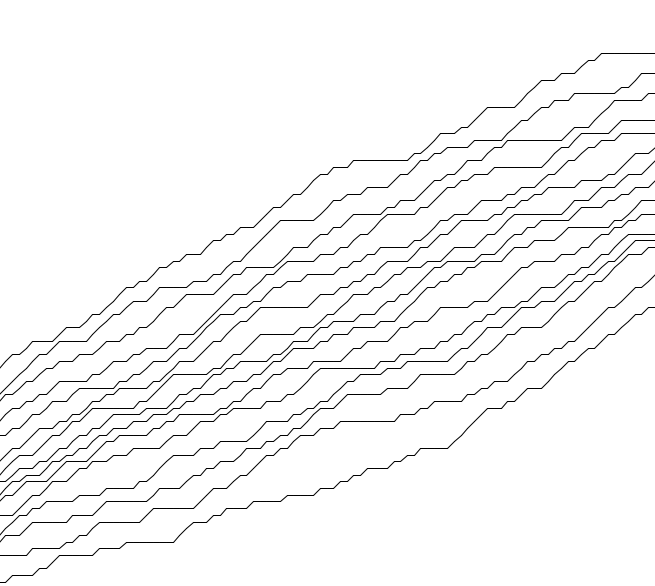
\includegraphics[height=0.25\textheight]{graphics/MultipleBernoulli.png}
	\caption{Multiple Bernoulli Random Walks}
\end{figure}
\begin{figure}
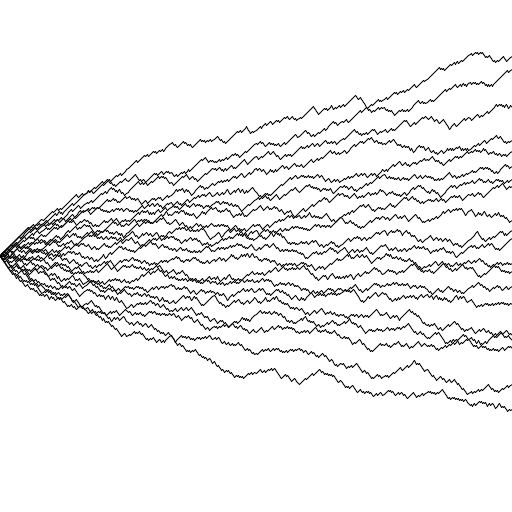
\includegraphics[height=0.25\textheight]{graphics/DysonBrownian.png}
\end{figure}
\end{frame}

\begin{frame}{Airy Line Ensemble}
What happens as N (number of walkers) goes to infinity? new type of limit occurs Airy line ensemble, top curve is the Airy process. Increasing the number of paths pushes us outside of the Gaussian universality class and into what is called the ”KPZ universality class”
\end{frame}

\begin{frame}{Open Question}
Big open problem: Show that for “generic random walks” with “generic” initial conditions we have convergence to Airy LE. This problem is open even for Bernoulli random walks (only known if all are started from 0)
\end{frame}


\section{Convergence to Airy Line Ensemble (6-7 min)}

\begin{frame}{Convergence to the Airy Line Ensemble}
	Two sufficient conditions:\begin{enumerate}
		\item Finite dimensional distribution convergence
		\item Tightness, or the existence of weak subsequential limits.
	\end{enumerate}
We focused on tightness, which requires a maximum, minimum, and conditions on the Modulus of Continuity
\begin{figure}
	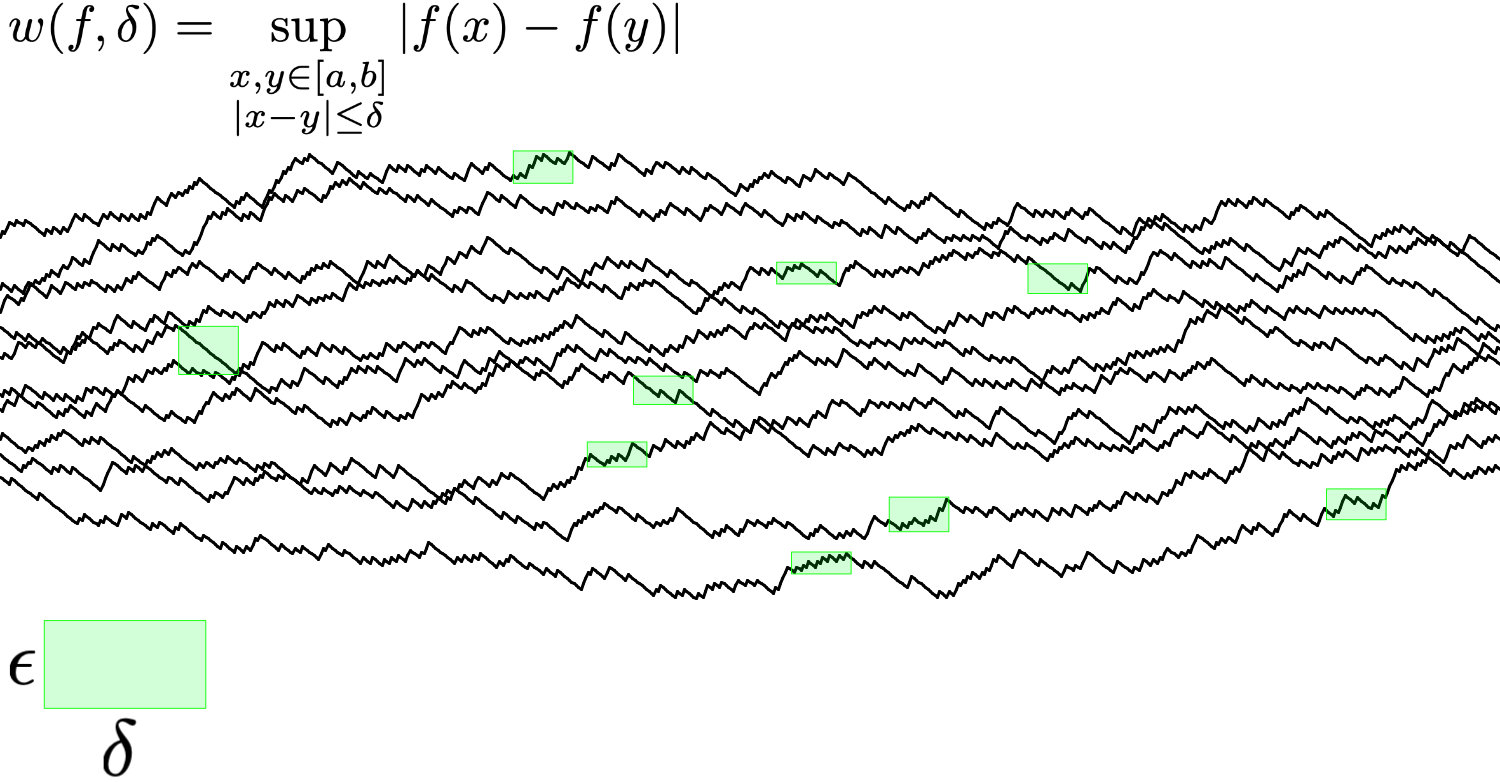
\includegraphics[height=0.55\textheight]{graphics/ModulusCont.jpg}
	\caption{The Modulus of Continuity}
\end{figure}

\end{frame}

\begin{frame}{Our Result}
Main result here: if top line 1 point marginals at integer times go to Tracy-Widom then the full LE is tight. 
$P(L_1^N(nN^{2/3}) - nN^{2/3} p + \lambda n^2 N^{1/3} \leq N^{1/3} x) \to F_{TW}(x)$
\begin{figure}
	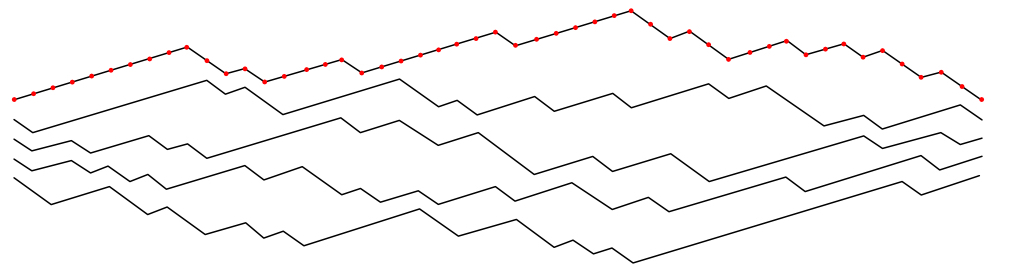
\includegraphics[width=\textwidth]{graphics/ConvToTW.jpg}
	\caption{Our result depends upon distribution points in red}
\end{figure}
\end{frame}

\begin{frame}{Previous Results}
Compare to Virag+Duavergne+Nica ‘19 (they assume fd convergence to Airy Line ensemble vs we assume only 1 point convergence of the top line to TW)
\end{frame}


\section{Section of Paper (7-9 min)}

\begin{frame}
Arguments are inspired by [Corwin-Hammond ‘14, ‘15] (continuous setting) [Corwin-Dimitrov ‘17] (discrete setting) Description of the problem ( min, max and modulus of continuity)
2 min   $P( \inf_{s\in[-r, r]} L_1^N(sN^{2/3}) - psN^{2/3}  < -RN^{1/3} ) < \epsilon$ if $R,N$ are large enough  
\end{frame}

\begin{frame}
Proof  (mention monotone coupling lemmas somewhere ) - say MC with picture
2min
\end{frame}

\begin{frame}
Proof  (mention strong coupling somewhere) - say SC with picture 
L = Bernoulli bridge B is a Brownian bridge with variance. There is a probability space such that $P( sup \abs*{L - B} \geq k (\log N)^2) < \epsilon$. This is a comparison that allows for example to compare the modulus of continuity of the two. [Dimitrov-Wu ‘19]
2 min
\end{frame}

\begin{frame}{Controlling the minimum: pinning the bottom curve}
	
	\begin{lemma}[------]
		For any $r,\epsilon > 0$, there exists $R>r$ and a constant $A>0$ so that for large $N$,
		\[
		\mathbb{P}\Big(\max_{x\in[r,R]} \big(L_k^N(xN^{2/3}) - pxN^{2/3}\big) \leq -AN^{1/3}\Big) < \epsilon.
		\]
		The same is true of the maximum on $[-R,-r]$.
	\end{lemma}
	
	
	
\end{frame}

\begin{frame}{Proving the pinning lemma}
	
	\begin{itemize}
		
		\item Recall our assumption:
		\[
		\mathbb{P}\Big(\textcolor{red}{L_1^N}(nN^{2/3}) - pnN^{2/3} + \textcolor{red}{\lambda n^2} N^{1/3} \leq xN^{1/3}\Big) \underset{N\to\infty}\longrightarrow F_{TW}(x).
		\]
		
	\end{itemize}
\end{frame}


\end{document}